\documentclass[12pt]{article}
\usepackage[utf8]{inputenc}
\usepackage{amsmath}
\usepackage{times}
\usepackage{amsfonts}
\usepackage{amssymb}
\usepackage{graphicx}
\usepackage{tabularx}
\usepackage[font=small,labelfont=bf]{caption}
%\usepackage[font=small]{subcaption}
\usepackage{wrapfig}
\usepackage{subfig}
\usepackage[american]{babel}
\usepackage{csquotes}
\usepackage{xcolor}
\usepackage[style=apa,backend=biber,sorting=none]{biblatex}
\DeclareLanguageMapping{american}{american-apa}
\usepackage[section]{placeins}
\usepackage{rotating}
\usepackage{bbm}
\usepackage{latexsym}


\DeclareSourcemap{
  \maps[datatype=bibtex]{
    \map{
      \step[fieldset=abstract, null]
    }
  }
}

\addbibresource{thesis.bib}
%\renewcommand\thesubsection{\alph{subsection}}


%\DeclareGraphicsExtensions{.eps,.png}

%%% margins 
\textheight 23.4cm
\textwidth 14.65cm
\oddsidemargin 0.375in
\evensidemargin 0.375in
\topmargin  -0.55in
%
\renewcommand{\baselinestretch}{2}
%
\interfootnotelinepenalty=10000
%
\renewcommand{\thesubsubsection}{\arabic{section}.\arabic{subsubsection}}
\newcommand{\myparagraph}[1]{\ \\{\em #1}.\ \ }
\newcommand{\parencitealtt}[1]{\parenciteauthor{#1},\parenciteyear{#1}}
\newcommand{\myycite}[1]{\parencitep{#1}}

% Different font in captions
\newcommand{\captionfonts}{\small \it}

\makeatletter  
\long\def\@makecaption#1#2{%
  \vskip\abovecaptionskip
  \sbox\@tempboxa{{\captionfonts #1: #2}}%
  \ifdim \wd\@tempboxa >\hsize
    {\captionfonts #1: #2\par}
  \else
    \hbox to\hsize{\hfil\box\@tempboxa\hfil}%
  \fi
  \vskip\belowcaptionskip}
\makeatother   
%%%%%

\begin{document}
\hspace{13.9cm}

\ \vspace{20mm}\\

{\LARGE Traveling waves in two-dimensional neuronal systems}

\ \\
{\bf \large Vincent Baker, vjb42@drexel.edu$^{\displaystyle 1}$}\\
{\bf \large Luis Cruz, ccruz@drexel.edu$^{\displaystyle 1}$}\\
{$^{\displaystyle 1}$Drexel University, Department of Physics.}\\
%

%\ \\[-2mm]
{\bf Keywords:} Traveling waves, one-dimensional networks, minicolumns, microcolumns, cortical organization, time delay, balanced excitation and inhibition

\thispagestyle{empty}
\markboth{}{NC instructions}
%
\ \vspace{-0mm}\\
%
%Abstract
\begin{center} {\bf Abstract} \end{center}
Traveling waves of neuronal activity in the cortex have been observed in vivo.
These traveling waves have been correlated to various features of observed cortical dynamics including spike timing variability and correlated fluctuations in neuron membrane potential.
Although traveling waves are typically studied as either strictly one-dimensional or two-dimensional excitations, here we investigate the conditions for the existence of quasi  one-dimensional traveling waves that could be sustainable in parts of the brain containing cortical minicolumns.
For that, we explore a quasi  one-dimensional network of heterogeneous neurons with a biologically influenced computational model of neuron dynamics and connectivity.
We find that background stimulus reliably evokes traveling waves in networks with local connectivity between neurons.
We also observe traveling waves in fully-connected networks when a model for action potential propagation speed is incorporated.
The biological properties of the neurons influence the generation and propagation of the traveling waves. 
Our quasi  one-dimensional model is not only useful for studying the basic properties of traveling waves in neuronal networks, but it also provides a simplified representation of possible wave propagation in columnar or minicolumnar networks found in the cortex.

%%%%%%%%%%%

\section{Introduction} 
Connected neurons that fire sequentially can stimulate firings from neighboring neurons, creating a traveling wave of neuron spikes. 
These traveling waves have been observed in the cortex of mammalian brains \parencite{Muller2018}\parencite{reimer2010}  as well as in vitro \parencite{wu2008}\parencite{huang2004}\parencite{Golomb1999}, and subsequently have been reproduced in silico \parencite{keane2015}\parencite{Senk2020}\parencite{Golomb1996}\parencite{ermentrout2001}. 
While the function of traveling waves is unknown \parencite{wu2008}\parencite{Muller2018}, proposed functions include motor coordination \parencite{Rubino2006}  , place field coordination in the hippocampus \parencite{lubernov2009}, and spatiotemporal processing in the visual cortex \parencite{wu2008}\parencite{Muller2014}.

Neuronal traveling waves are not uniquely defined as they can exist at widely differing frequency and scale lengths.  
In the sleep and anesthetized states,slow and large-scale wave activity has been recorded \parencite{Muller2018}. 
Traveling waves have been detected in local-field potentials measured with electrodes \parencite{Rubino2006}\parencite{sanes1993}\parencite{Riehle2013}.
Local-area traveling waves in the awake cortex have been observed using recent advances in optical imaging techniques using voltage-sensitive dyes \parencite{wu2008}\parencite{Shoham1999}\parencite{Xu2007}\parencite{Ferezou2006}.  
Similarly, traveling waves also differ by the manner in which they are created. 
Both spontaneously occurring waves and stimulus-evoked \parencite{reimer2010} waves have been observed in the visual and auditory cortex. 
Computational and mathematical modeling of traveling waves in a variety of models have shown many of the characteristics observed experimentally \parencite{ermentrout2001}\parencite{keane2015}\parencite{gibson2009}.

Studies of traveling waves have focused on two-dimensional waves that spread parallel to the surface (pia) of the brain \parencite{reimer2010}\parencite{keane2015}\parencite{Townsend2018}\parencite{Golomb1997}\parencite{Qi2015}. 
This is to be expected as this is the geometry of the system on which they are observed, and \parencite{Wilson1973} provide an anatomical argument for focusing on such structure. 
Traveling waves in one-dimensional neuronal systems have been previously explored using several theoretical methods.
In the literature on neural fields \parencite{Ermentrout1979}\parencite{Folias2012} and coupled oscillators \parencite{Kopell1986}\parencite{Williams1997} isotropic networks of homogeneous neurons with symmetric synaptic coupling give rise to field models which exhibit traveling wave solutions for certain parameter values. 
One-dimensional waves have also been observed in simulations using firing rate neurons \parencite{Roxin2005}, integrate-and-fire neurons \parencite{Bressloff1997}\parencite{Golomb1999} and Hodgkin-Huxley neurons \parencite{Golomb1997}.
\parencite{Senk2020} used populations of both rate neurons and integrate-and-fire neurons and developed a method to translate parameters between the two different models.

These simulations again use homogeneous neuronal populations in networks that are invariant to spatial translation, resulting naturally in periodic spatio-temporal patterns.
These purely one-dimensional systems may not be robust to realistic variation in neuron properties, connectivity and noise.
This is exemplified in \parencite{Senk2020} where traveling waves are only observed for certain parameter values, and \parencite{Strogatz1991} where the stability of systems of coupled oscillators can be radically altered by including infinitesimal noise.
Our current work explores traveling waves in quasi-one-dimensional networks with substantial randomness in both individual neurons (randomly selecting type and randomizing dynamical parameters), connectivity between neurons, and stimulus to the neurons.

Previous studies have used one-dimensional structures largely for their computational or analytic simplicity. 
Consideration of a quasi one-dimensional system may seem as an unnecessary complication, but there is no a priori reason that quasi one-dimensional traveling waves may not be found in vivo.
Of interest, there are regions of the brain where there are what seem to be quasi  one-dimensional structures \parencite{buxhoeveden2002}\parencite{mountcastle1997} typically called micro- or minicolumns. 
These minicolumns are aligned perpendicular to the pia and can be hundreds of microns long.  
Although their relevance to cognition and function is still being debated \parencite{horton2005}\parencite{Cruz2009}\parencite{buxhoeveden2002}, it is possible that they can sustain traveling waves.

To address this possibility, here we investigate the conditions under which traveling waves can exist on quasi one-dimensional systems, and their fundamental properties and dynamics.  
Inspired by minicolumns, our systems consist of thin (few neuron) and long (~100 neuron) networks of locally connected neurons placed on a three-dimensional lattice.  
We model the neuron dynamics using the Izhikevich model \parencite{izhikevich2003} that allow us to explore more complex neuron dynamics than typically afforded by integrate-and-fire models \parencite{keane2015}\parencite{Senk2020} while also providing a distribution of neuron dynamical parameters that mimics the type and variety of neurons observed in the mammalian cortex.
We use a morphology and connectivity model inspired by \parencite{maass2002},incorporating a local connectivity model \parencite{Levy2012}\parencite{Pyle2017}\parencite{Fino2011}.
To incorporate elements of a real brain, we consider a model with substantial randomness in both individual neurons and connections between neurons while also considering  distance-dependent time delays in the propagation of action potentials.

Among our main findings we determine parameters in our model that allow for the generation of traveling waves in our quasi one-dimensional systems. 
These traveling waves exhibit properties such as spontaneous creation from a random background stimulus, annihilation of colliding waves, and a wave velocity that is determined by both the propagation speed of the action potential and the neuron dynamics.
Traveling waves are present in both locally-connected and fully-connected systems. 
The traveling waves in fully connected systems are dependent upon the action potential propagation speed, while traveling waves can propagate in locally-connected systems even when action potential propagation is instantaneous.

Studies of traveling waves have focused on two-dimensional waves that spread parallel to the surface (pia) of the brain \parencite{reimer2010}\parencite{keane2015}\parencite{Townsend2018}\parencite{Golomb1997}\parencite{Qi2015}. 
This is to be expected as this is the geometry of the system on which they are observed, and \parencite{Wilson1973} provide an anatomical argument for focusing on such structure. 

We now expand our study of traveling waves in quasi 1-D minicolumns to two-dimensional topologies.
First we study two-dimensional sheets of neurons extended in the X and Y directions.
As before, we find that our model doesn't support traveling waves in a purely two-dimensional sheet (Z=1) under the model parameters studied.
When we extend the system to a quasi two-dimensional sheet (Z=2) we find traveling waves are evoked by both the background and impulsive stimulus.
We observe several types of waves in our sheets that match those observed in vivo, and demonstrate how model parameters shape the types of waves present in the system.
Our systems exhibit spatiotemporal attractor states, repeating patterns characterized by highly regular inter-spike intervals.
Two identical systems can settle into different attractor states depending on the stimulus applied.


\section{Methods}

\subsection{Neuron model}
Computational neuroscience makes use of a number of neuron models.
By far the most common model used when studying traveling waves and other mesoscopic behavior is the leaky integrate-and-fire neuron.
The computational efficiency of the LIF model has allowed researchers to simulate large numbers of neurons over time scales of seconds or minutes.
However this computational efficiency comes at the cost of accurate representation of internal neuron dynamics.
\\
The LIF equations model a single neuron variable, the membrane potential, in a single differential equation.
The Izhikevich model includes an additional variable that represents a collection of ionic mechanisms and uses two coupled differential equations.
This two-dimensional model can capture a number of biologically observed dynamical phenomenon not possible in a one-dimensional model while still being computationally efficient.
\\
Critical phenomenon observed in the Izhikevich model and not the LIF model include variable firing rates, post-inhibitory rebound spiking and delayed spiking.
Plots: LIF vs Izzy post-inhibitory rebound spiking, delayed spiking, 

To study traveling waves in small columnar ensembles (SCE) of neurons we created a MATLAB simulation of our model based on \parencite{izhikevich2003}.
We model the firing dynamics of each neuron using the Izhikevich model \parencite{izhikevich2003} that consists of a two-dimensional model of two coupled differential equations given by:
\begin{align}
 \begin{split}
  v^\prime &= 0.04v^2+5v+140-u+I \label{eq:neuron_v} \\
  u^\prime &= a(bv-u)
 \end{split}
\end{align}
where $v$ is the membrane potential of the neuron and $u$ is a membrane recovery variable, with a spike threshold and an auxilliary after-spike resetting of parameters by:
\begin{align}
  \text{if } &v>30: v\leftarrow c, u\leftarrow u+d
\end{align}
and I is the sum of all incoming currents to the neuron, explained in detail below. 

Equation \ref{eq:neuron_v} has four parameters (a,b,c,d) that with specific values can model a wide range of neuronal spiking behavior \parencite{izhikevich2003}. 
The parameters used here (see Table \ref{tab:izzy_params}) are based on the original model with modification of the $c$ parameter for excitatory neurons and define a random population of neurons where $U(s,t)$ represent a number drawn from a uniform random distribution between s and t. 
\begin{table}[!htb]
 \caption{Izhikevich model parameters}
 \label{tab:izzy_params}
 \centering
 \begin{tabular}{lcr}
  \textbf{Parameter} & \textbf{Excitatory} & \textbf{Inhibitory} \\
  \hline
  a & 0.02 & 0.02+$\mathcal{U}$(0,0.08) \\
  b & 0.2 & 0.25-$\mathcal{U}(0,0.05)$\\
  c & -65+$\mathcal{U}(0,10)^2$ & -65 \\
  d & 8-$\mathcal{U}(0,6)$& 2 \\
 \end{tabular}
\end{table}
For solving equation \ref{eq:neuron_v} numerically we use the modified Euler method from \parencite{izhikevich2003} with a time step of $0.2 ms$ except were noted. 

The current I in equation \ref{eq:neuron_v} includes the sum of all incoming stimuli into neuron $i$ from other neurons $I_i$ and external stimuli $I_{i,e}$ applied to the system. 
The neuron-neuron incoming current $I_i$ into neuron $i$ is given by:
\begin{align}
 I_i(t) &= \sum_{j\ne i} \sum_{t^\prime_j} S_{ij}  \Theta(t-t^\prime_j-\tau_{ij})e^{-(\frac{t-t^\prime_j-\tau_{ij}}{\sigma_s})^2}
\end{align}

where $t'_j$ are the firing times of neuron $j$, $\Theta$ is the Heaviside step function, and the exponential factor models an exponentially decaying synapse response with a time constant of $\sigma_s = 4 ms$. 
The $S_{ij}$ represent the connection strengths between presynaptic neuron $j$ and postsynaptic neuron $i$ given by
\begin{align}
 \begin{split}
  S_{ij}^{excitatory} &= K \times \mathcal{U}\{0,0.5 \} \\
  S_{ij}^{inhibitory} &= K \times \mathcal{U}\{-1,0 \}  \\
 \end{split}
\end{align}
where $K$ is a parameter that modulates the strength of connections, with $K=1$ corresponding to the original model in \parencite{izhikevich2003}. 

The distribution of Izhikevich model parameters results in variations between our excitatory and inhibitory neurons, as well as variation in the neurons within those classes.
We examine the inter-spike interval (ISI) and its inverse, the spike frequency, for the excitatory and inhibitory neurons in our model.
We generate 1600 excitatory or inhibitory neurons and drive them with a constant stimulus, measuring the resulting ISI/spike rate as shown in Figure \ref{fig:ISIstatistics}.
The inhibitory neurons spike at a lower input level and the spike rate rises more quickly with stronger input.
Due to the stochastic variation in the 'b' parameter for inhibitory neurons, different inhibitory neurons can have a different minimum firing threshold.
Starting at an input magnitude of $4\ mV$, at which all the inhibitory neurons fire, the spike rate of the inhibitory neurons increase linearly with the input magnitude with a slope of 13.
The excitatory neurons all have a common firing threshold.
The spike rate of the excitatory neurons increases linearly with the input magnitude, and the slope of the linear fit is 3.
\begin{figure}[!htb]
  \subfloat[][]{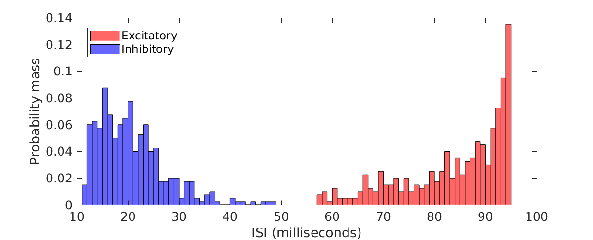
\includegraphics[width=0.75\textwidth]{fig/ISIDistribution} } \\
  \subfloat[][]{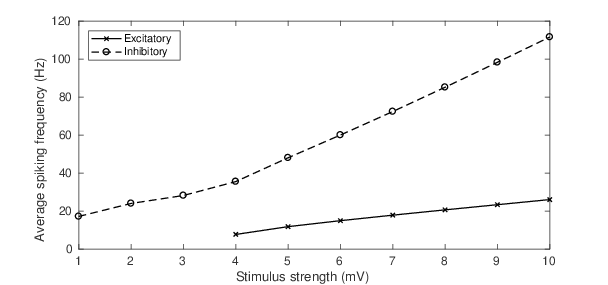
\includegraphics[width=0.75\textwidth]{fig/AvgSpikeFrequency} }
  \caption{a) The distribution of inter-spike intervals for our excitatory and inhibitory neurons with a constant $5\ mV$ stimulus.  
      b) The spike frequency of the excitatory and inhibitory neurons increases as the constant stimulus becomes stronger.}
  \label{fig:ISIstatistics}
\end{figure}
\FloatBarrier

\subsection{Neuron stimulus}
To drive the firing dynamics and create traveling waves we provide stimulation to the systems by using two different and separate external stimulus currents, $I_{i,e}$. 
One of them is a uniform background stimulus applied to each neuron $k$ that depends on whether the neuron is excitatory or inhibitory.
The stimulus values are drawn from a random distribution every $1 ms$ according to:
\begin{align}\label{eq:randomstim}
 \begin{split}
  I_k^{excitatory} &= M \times \mathcal{U}\{0,1 \} \\
  I_k^{inhibitory} &= \frac{2}{5} M \times \mathcal{U}\{0,1 \}
 \end{split}
\end{align}
where $M$ is a parameter that tunes the overall strength of the stimulus, with $M=5$ corresponding to the original model in \parencite{izhikevich2003}. 
This stimulus has the effect of creating waves that originate from any point along an SCE and one of the uses is to study interactions between multiple waves.

The other external stimulus $I_{i,e}$ is a short constant input of current applied to all of the neurons in one area of a system.
This stimulus is used to measure wave speed.

\subsection{Neuron connectivity}
We first construct these assemblies by placing neurons at the vertices of a cubic lattice with coordinates X, Y and Z. 
Each neuron is  randomly chosen to be  either excitatory (E) or inhibitory (I), with the fraction of excitatory neurons indicated as $P_{exc}$.
After placing, we connect two neurons based on their relative distance according to a connection probability that favors local connectivity given by \parencite{maass2002}: 
\begin{align}\label{eq:connectivity}
 P_{a,b} &= C e^{-(D(a,b)/\lambda)^2}
\end{align}
where $D(a,b)$ is the Euclidean distance between neuron a and b, $\lambda$ is the characteristic length of the local connectivity neighborhood, and $C$ is the peak probability of connection.
This local connectivity model has been observed in the mouse visual cortex\parencite{Hellwig2000} and auditory cortex\parencite{Levy2012}.
Multiple connections from the same presynaptic neuron to the same postsynaptic neuron, as well as self-connections, are prohibited.
Two neurons may be recurrently connected, however. 

\subsection{2-D topologies}
Each sheet consists of neurons placed on a unit grid. 
The X and Y extents are much larger than the Z extent.
We generally use sheets with Z=2 with the exception of one purely two-dimensional example with Z=1.
Neurons are created and connected as described in Methods.
Due to the larger area of regard and the more demanding computational experiments we use periodic boundary conditions in our quasi two-dimensional sheets.
A small example quasi 2-D sheet is shown in Figure \ref{fig:sheet_structure}.
In this small example the periodic boundary conditions are easily seen as multiple diagonals in the connection matrix.

\begin{figure}[!htb]
 \caption{Example small quasi 2-D sheet with dimensions X=10, Y=10, Z=2. The connection parameters are set to $\lambda$=2.5 and C=0.5. 
 a)  Sheet showing connections between neurons as lines colored using a color scale that indicates the connection length. 
 b)  Connection matrix. E-E connections are green, E-I are black and both I-E and I-I  are red. 
 c) The sum of presynaptic weights for each neuron shows the anisotropy of this model, with substantial variation in input strength and sign between the neuron inputs.}
 \label{fig:sheet_structure}
 \subfloat[][]{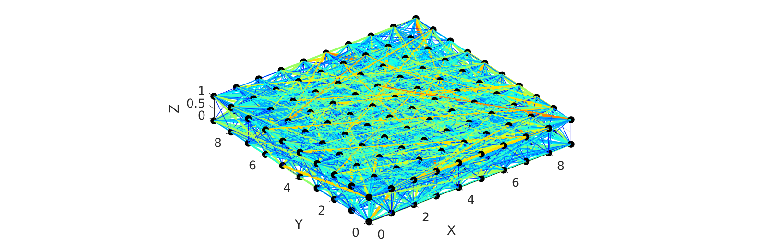
\includegraphics[width=\textwidth]{fig/Sheet_Structure_A}}\\
 \subfloat[][]{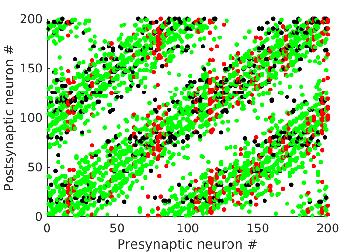
\includegraphics[width=0.5\textwidth]{fig/Sheet_Structure_B}}
 \subfloat[][]{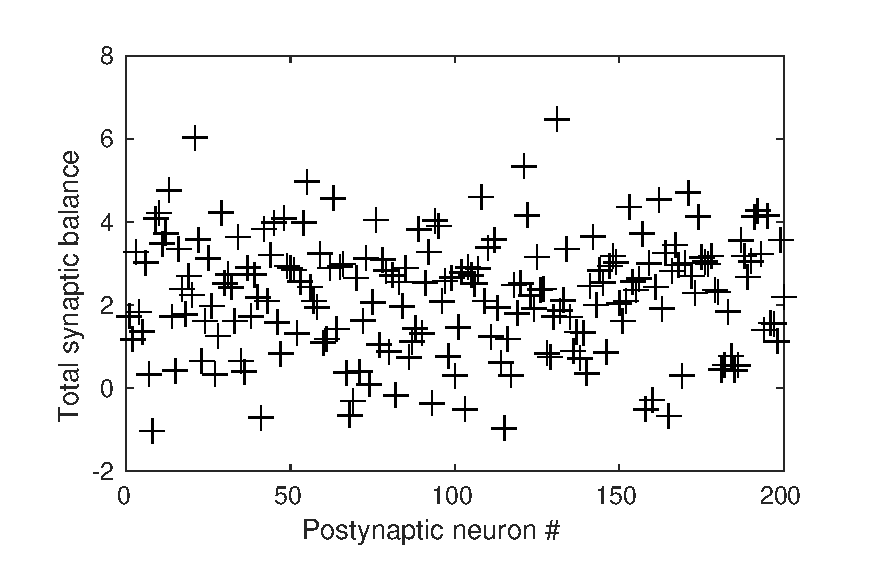
\includegraphics[width=0.5\textwidth]{fig/Sheet_Structure_C}}
\end{figure}

The topology of our sheet combined with our local connectivity rule (eq. \ref{eq:connectivity}) defines the connection distribution of the sheet.
The distribution of post-synaptic connections and delay times are shown in Figure \ref{fig:connection_delay_distrbution_2D} for an example quasi 2-D sheet.
\begin{figure}[!htb]
 \caption{Distribution of (a) number of post-synaptic connections per neuron and (b) delay time. 
          Data was taken from an X=100, Y=100, Z=2 sheet with $\lambda=2.5$, $\kappa=1$ and periodic boundary conditions.  } 
     \subfloat[][]{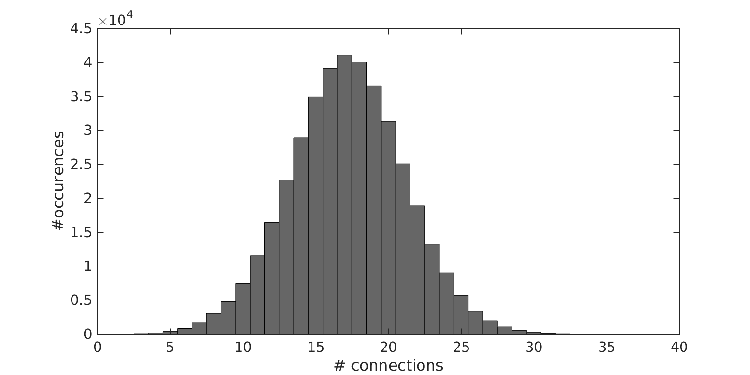
\includegraphics[width=0.48\textwidth]{fig/ConnectionNumberDistribution2D} }
     \subfloat[][]{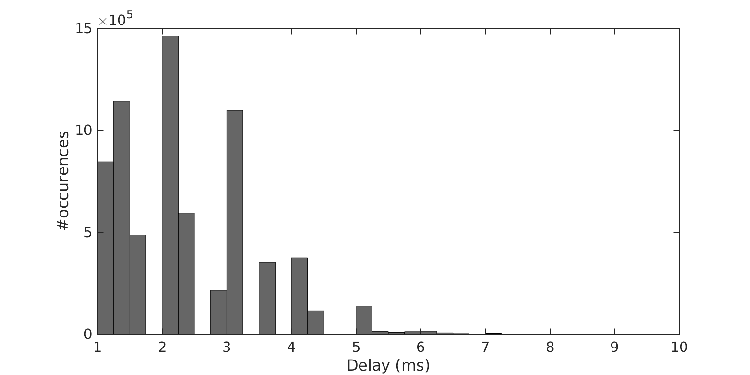
\includegraphics[width=0.48\textwidth]{fig/DelayDistribution2D} }
 \label{fig:connection_delay_distrbution_2D}
\end{figure}
 \FloatBarrier

\subsection{Model summary}
We summarize our model parameters in Table \ref{tab:all_params}. 
\begin{table}[!htb]
 \caption{Model Summary}
 \label{tab:all_params}
 \centering
 \begin{tabular}{c}
  \textbf{Model} \\
  \hline \\
 \end{tabular} \\
 \begin{tabular}{ll}
  Population & Excitatory, inhibitory \\
  Topology & Quasi 1-D minicolumn, quasi 2-D sheet, ``2.5D'' forest of minicolumns \\
  Connectivity & Stochastic, $P_{connect}$ exponentially decays with distance between neurons \\
  Neuron model & Izhikevich model with distribution of neuron parameters \\
  Synapse response & Exponential synaptic response with randomized peak connection strength  \\
  Spike propagation & Delay proportional to distance, Fixed propagation time \\
  Input & Random input to all neurons, Fixed stimulus to neurons at the bottom of the SCE \\
 \end{tabular}
\end{table}

\subsection{Wave speed measurements}\label{sec:wave_speed_method}
To measure wave speeds we apply a constant stimulus $I_{i,e}$ over a short time period to a local area of the system.
There is no stimulus to the other neurons in the system.
This short stimulus initiates a single traveling wave that spans the entire system.
The wave arrival time is measured at some reference point in the system, and the wave speed is calculated from the wave arrival time and the distance the wave travels.

For the minicolumn system $I_{i,e}$ has a magnitude of $5$ units and is applied to the lowest $10$ layers of the minicolumn for $20~ms$.
The one-dimensional waves travel in the Z direction and the wave arrival time is measured at the top of the minicolumns.
For the two-dimensional sheet $I_{i,e}$ has a magnitude of $5$ units and is applied for $10~ms$ to the neurons at X=\{0,1\}, Y=\{0,1\} and Z=\{0.1\} in the lower left corner of the sheet.
The waves span the entire sheet in both the X and Y directions, and the wave arrival time is measured at the lower right edge (Y=0, X at maximum value). 
For the forest of minicolumns $I_{i,e}$ has a magnitude of $5$ units and is applied for $10~ms$ to the single minicolumn in the lower left corner of the forest.
The stimulus evokes waves that travel in the X/Y plane and the wave arrival time is measured at the minicolumn in the lower right corner of the forest.

\subsection{Spike correlation analysis}\label{sec:spike_correlation_analysis}
For our quasi two-dimensional systems we characterize the spatio-temporal activity using the inter-spike interval (ISI), the coefficient of variation (CV) of the ISI, 
and the cross-correlation of the spike counts between neurons.
The distribution of the ISI reveals temporal patterns in our quasi-2D systems.
The CV of the ISI indicates the temporal regularity of the spiking activity, where a CV of $0$ indicates perfectly regular repetitaion while a Poisson process
has a CV of $1$.
We calculate the cross-correlation between neuron spike counts as a function of the distance between neurons.
This measure can reveal local correlations in firing activity indicative of traveling waves.
These measures were used by \parencite{keane2015} to show that traveling waves could simultaneously explain both the irregular firing of individual neurons
and the correlated firing between nearby neurons.

The CV of the ISI is calculated as:
\begin{align}\label{eq:cv}
 CV_{i} &= \frac{\sqrt{\textbf{var}(X_{i})}}{\langle X_{i} \rangle}
\end{align}
where $X_{ij}$ is the vector of all the inter-spike intervals from a simulation.

The cross-correlation of the spike counts between neurons $i$ and $j$ is goven by:
\begin{align}\label{eq:cross_correlation}
 CC_{i,j}(\tau) &= \frac{ \sum_{l=1}^L (N_i(t^l)-\langle N_i(t^l) \rangle) (N_j(t^l+\tau)-\langle N_j(t^l) \rangle) } { \sqrt{\text{var}(N_i(t^l))\text{var}(N_j(t^l))}  }
\end{align}
where $L$ is the total number of samples in time time series and the spike counts are summed over $50~ms$ windows stepped at $1~ms$ intervals.
In our simulations it is common for a neuron to not spike within a $50~ms$ interval.
We therefore modify this metric and do not normalize by the variance to avoid division by $0$.
Here we are only interested in the zero-lag cross-correlation at $\tau=0$ as we want to determine if the firing activity of nearby neurons is correlated.

\subsection{Wave Analysis}

A basic test of the wae analysis method is shown in figure \ref{fig:WavePropTest}.
The test data includes a single well defined spreading wave.
We performed the wave analysis for neurons under test along the diagonal from $x=y=150$ to $x=y=160$.
For each $x,y$ position we compared the estimated wave direction and speed for the neurons at $z=0$ and $z=1$.
The wave direction difference (mean $2.8$ degrees, standard deviation $6.1$ degrees) and the wave speed difference (mean $0.065$ units/ms, standard deviation $0.097$ units/ms)
indicate that the wave property measurement method is consistent.
Furthermore, the wave direction (around $224$ degrees) and speed (around $0.8$ units/ms) measured across all ten $x,y$ locations was consistent with visual inspection of the wave.

\begin{figure}[!htb]
 \caption{Example of wave analysis.
          a) Spike raster plot of the test data, showing a well-defined spreading wave starting at $t=1100~ms$ around $(90,180)$.
             The test positions are shown with red dots.
          b) Plot showing the spike time difference from the neuron under test as a function of the spatial offset. The neuron under test is at position $x=160$, $y=160$. $z=0$.
          c) Error when fitting the plane wave model to the data. The best fit is a wave direction of $226$ degrees, and the best fit wave speed was $0.8$ units/ms.
          } 
     \subfloat[][]{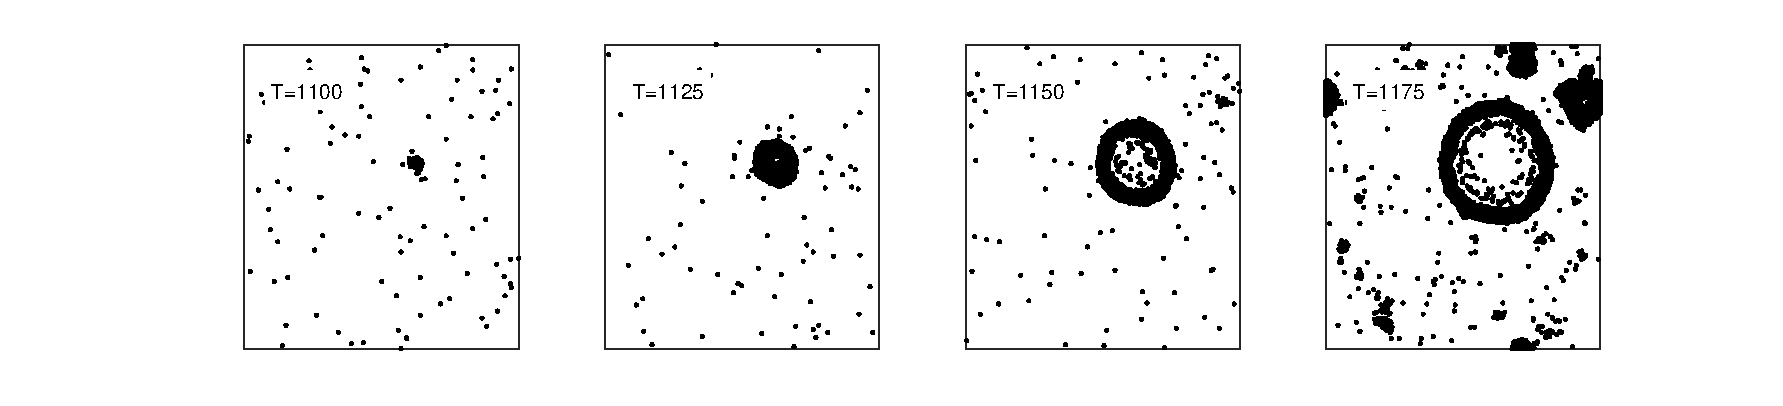
\includegraphics[width=\textwidth]{fig/WavePropTest_Rasters} } \\
     \subfloat[][]{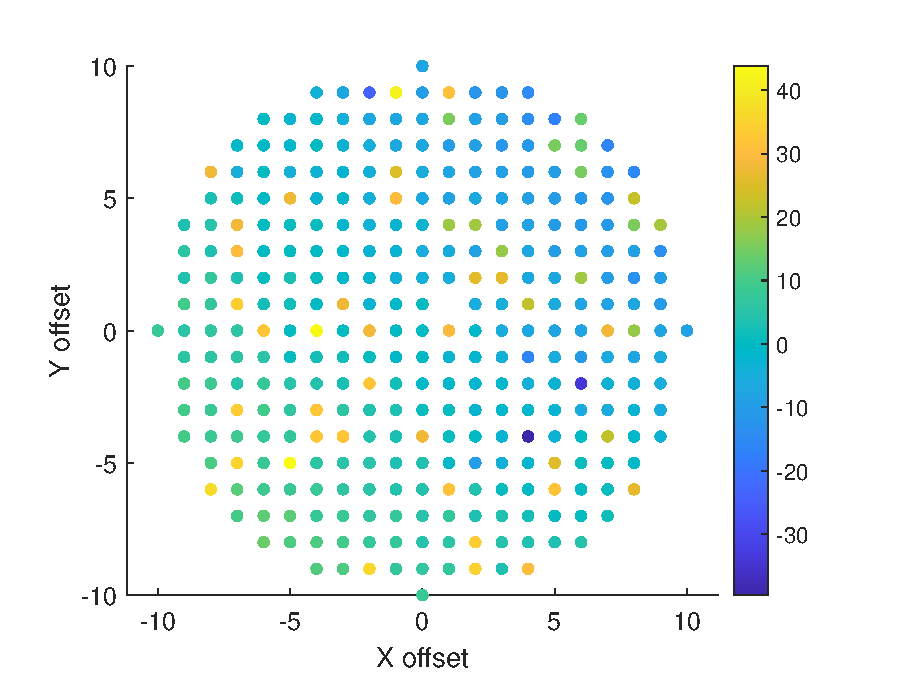
\includegraphics[width=0.48\textwidth]{fig/WavePropTest_SpikeDelays} }
     \subfloat[][]{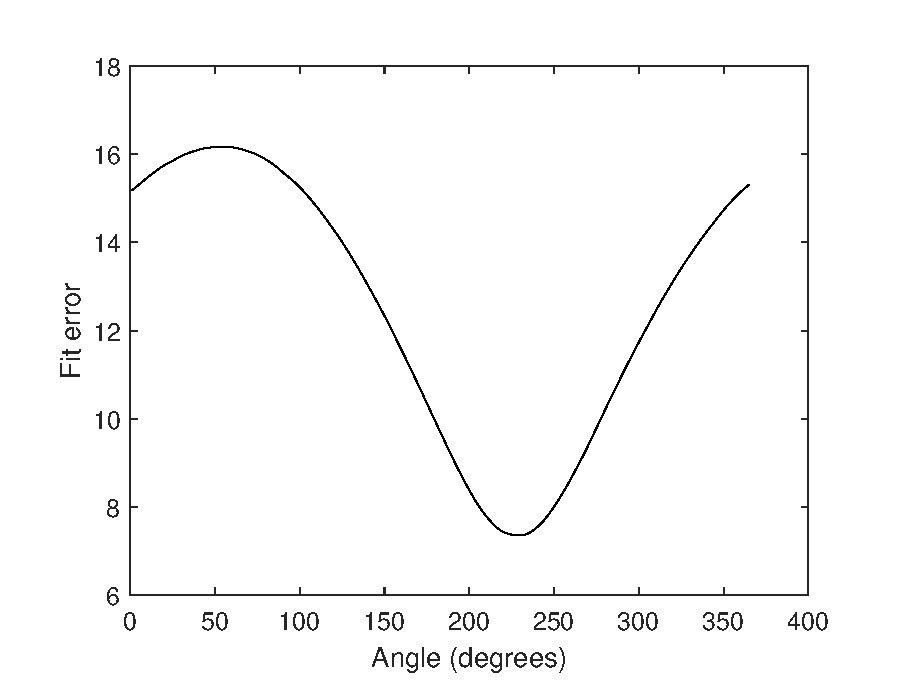
\includegraphics[width=0.48\textwidth]{fig/WavePropTest_AngleFittingError} }
 \label{fig:WavePropTest}
\end{figure}
\FloatBarrier


\section{Results}
We first create a purely 2-D sheet of neurons with X=300, Y=300 and Z=1.
Model parameters are fixed at $\Sigma$.
We do not observe traveling waves in this system (Figure \ref{fig:Pure2DRasters_NoWaves}).
\begin{figure}[!htb]
 \caption{Sequential frames showing the average membrane voltage in the X-Y plane.
          The system dimensions are 300x300x1, model parameters are at $\Sigma$. 
	  A 5x5 smoothing filter has been applied to this and all similar figures to enhance the spatiotemporal structure.}
 \label{fig:Pure2DRasters_NoWaves}
 \centering
   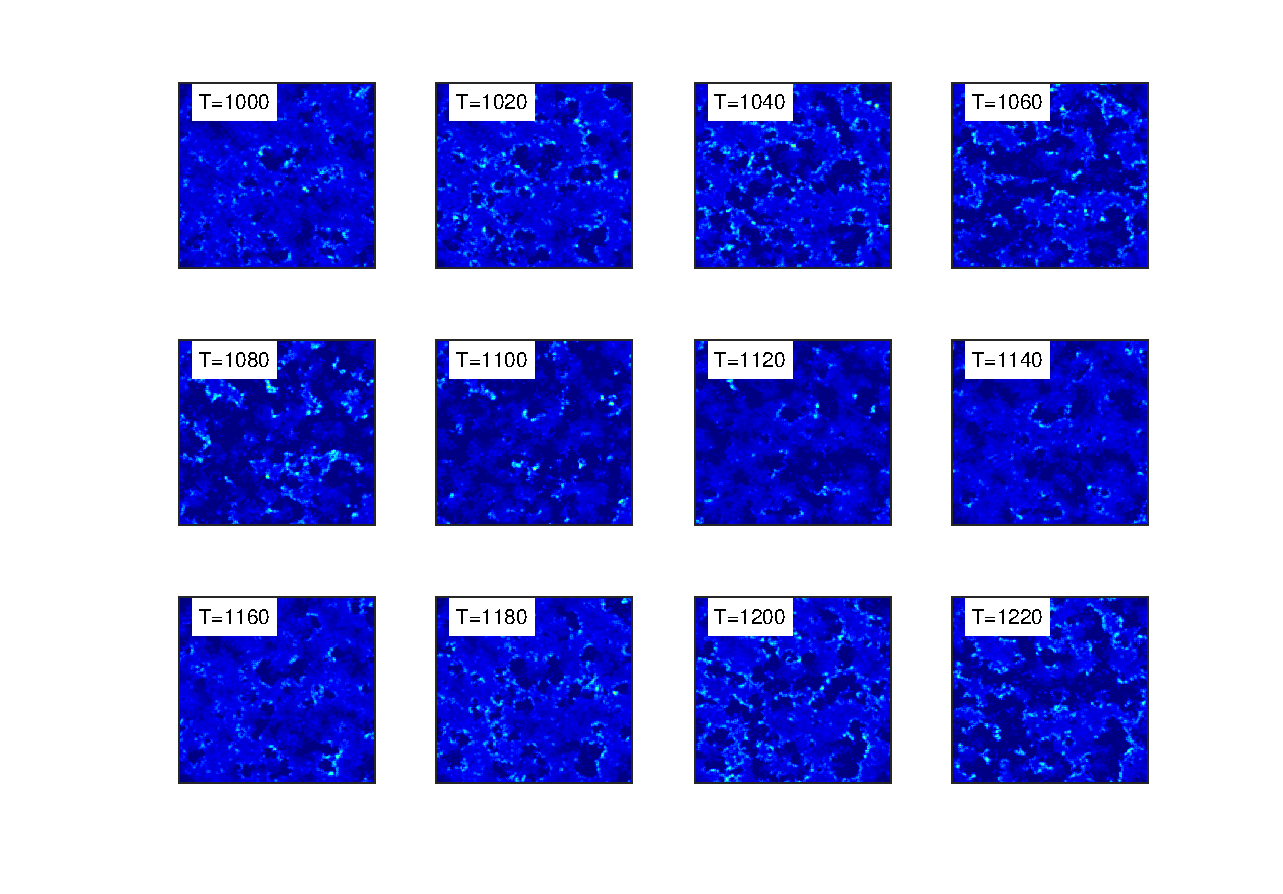
\includegraphics[width=\textwidth]{fig/2D_1LayerNoWaves}
\end{figure}
\FloatBarrier

We do observe a local spatial organization in the activity with nearby neurons tending to fire together.
However this locally coordinated firing activity does not result in traveling waves.
We also see a temporal rhythm with periods of higher and lower activity.
To quantify the temporal rhythm we calculate the inter-spike intervals for every neuron in the simulation.
The distribution of the inter-spike intervals is shown in figure \ref{fig:2D1LayerRhythm}.
\begin{figure}[!htb]
 \caption{The distribution of inter-spike intervals shown on a log scale shows a temporal pattern.
          There is a peak around $180~ms$ with smaller peaks near multiples of $180~ms$.
         }
 \label{fig:2D1LayerRhythm}
 \centering
   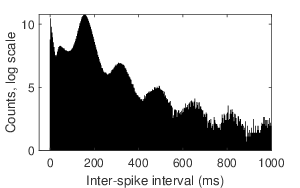
\includegraphics[width=0.6\textwidth]{fig/2D_1Layer_ISI_log}
\end{figure}

\FloatBarrier

We then extend our system to a quasi 2-D sheet with X=300, Y=300 and Z=2.
We now observe traveling wave patterns in the system.
These patterns emerge in spite of the high variability in the neuron types, neuron dynamics and connectivity present in our model.
We can clearly see  circular spreading waves emanating from multiple points within the sheet \ref{fig:2D_waves}.
These types of spreading waves have been observed in vivo\parencite{Mohajerani2013} and and in vitro, and can be spontaneously generated or evoked by a stimulus\parencite{Stroh2013}.
We observe repetitive patterns, most obviously a large wave emanating from the right side every $250~ms$.
The firing activity in the beginning of the simulation showed more variation, but the large circular wave comes to dominate the firing activity 
in a winner-take-all process due to wave annihilation.
\begin{figure}[!htb]
 \caption{ Wave patterns spreading across the surface of a sheet. 
           The system dimensions 300x300x2, model parameters are at $\Sigma$. 
           Circular spreading waves are evident, especially emanating from a point on the right side of the system.}
 \label{fig:2D_waves}
 \centering
   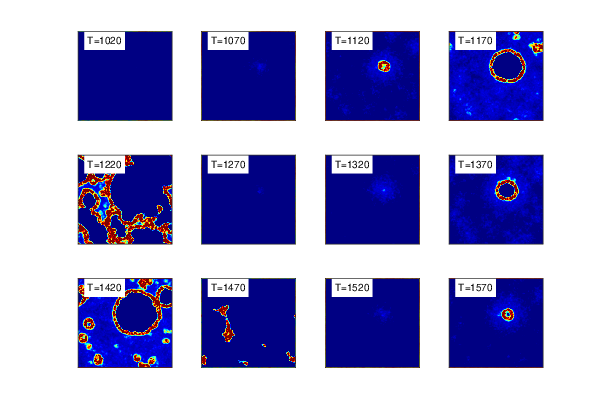
\includegraphics[width=\textwidth]{fig/2DSpreadingWaves_Sigma}
\end{figure}

\FloatBarrier

In some simulations we see the formation of large-scale plane waves across the entire system as seen by \parencite{keane2015}.
In their work, plane waves were formed when excitation dominated their neuronal system.
These plane waves seem to form due to the interaction of spreading circular waves.
The formation of plane waves in our system does not seem deterministic, as a different random draw of the uniform background stimulus for the same neuronal system may not exhibit plane waves.
Nonetheless, these results show that plane waves can emerge as a stable pattern in systems of this type even when excitation does not dominate.
\begin{figure}[!htb]
 \caption{ A plane wave front forming from multiple circular spreading waves.
          The system dimensions are 300x300x2, model parameters are at $\Sigma$.
          }
 \label{fig:2D_plane_wave}
 \centering
   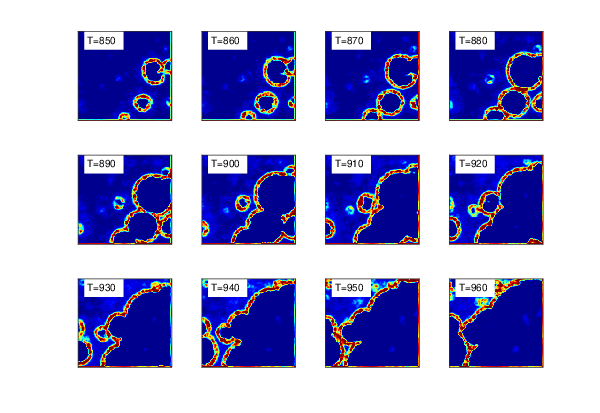
\includegraphics[width=\textwidth]{fig/2DPlaneWave}
\end{figure}
\FloatBarrier

We do not observe spiral waves in our simulations with the model parameters set at $\Sigma$.
With the higher connectivity observed in the sheet (figure \ref{fig:connection_delay_distrbution_2D}) we see circular waves emanating from a point.
Although these waves can combine to form a plane wave structure (figure \ref{fig:2D_plane_wave}), we do not observe spiral wave patterns across many simulations.
We reduce the connection strength K from $K=10$ to $K=6$.
The waves at the lower connection strength are thinner and sparser.
We now observe the formation of spiral wave pattern as seen in figure \ref{fig:2DSpiralWaves}.
\begin{figure}[!htb]
 \caption{ Spiral waves are apparent in the average membrane potential observed in a 2D sheet over time. 
           The system dimensions are 300x300x2. Model parameters are at $\Sigma$ except that $K=6$, $\kappa=0.1$.
           }
 \label{fig:2DSpiralWaves}
 \centering
   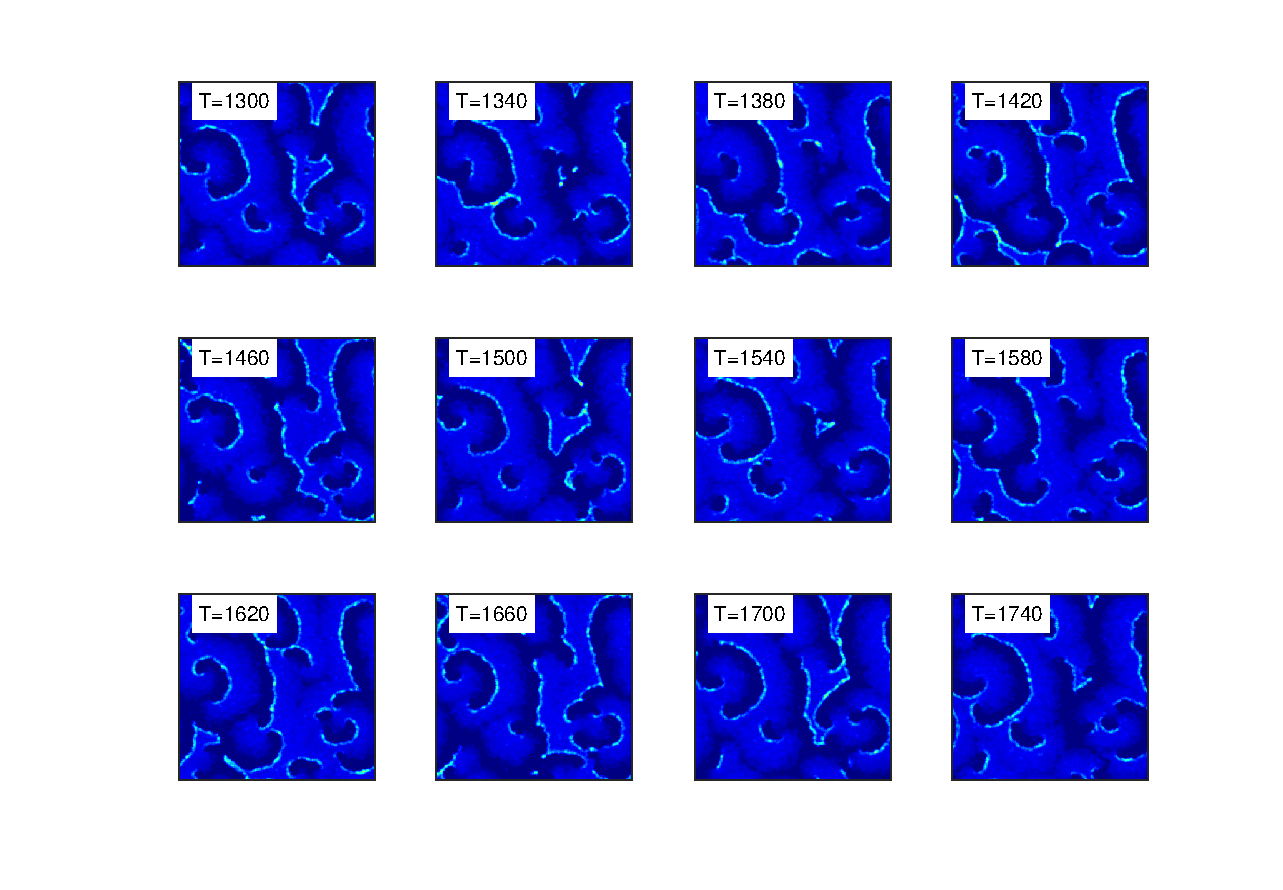
\includegraphics[width=\textwidth]{fig/SpiralWaves2D_K6_kappa0p1_M4}
\end{figure}
\FloatBarrier

\parencite{Huang2010} provide the observation that a plane wave with limited extents can generate a spiral wave pattern.
The firing activity at the edge of the plane wave will spread in directions that are not parallel to the plane wave propagation.
We observe similar behavior when the propagation of a circular spreading wave is not isotropic.
In this case we can see spiral waves shed from both edges of the circular wave as seen in figure \ref{fig:2DHeartWaves}.
We term these 'heart' waves.
\begin{figure}[!htb]
 \caption{ Spiral 'heart' waves are apparent in the average membrane potential observed in a 2D sheet over time. 
           The sheet is 200x200x2 with periodic boundary conditions, $K=6$, $\kappa=0.1$.
           }
 \label{fig:2DHeartWaves}
 \centering
   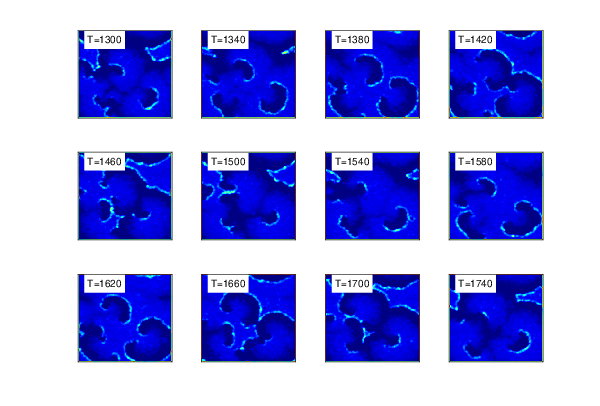
\includegraphics[width=\textwidth]{fig/2DSpiralWaves_HeartWaves}
\end{figure}
\FloatBarrier

We further examine the transition from spreading waves to spiral waves as connection strength decreases.
We hypothesize that the lower connection strength creates anisotropy that can disrupt a spreading wave propagation, resulting the heart and spiral patterns. 
We demonstrate this using a 100x100x2 sheet with a step stimulus as described in section \ref{sec:wave_speed_method}.
The stimulus is applied to the neurons at the center of the sheet at $t=0$ and generates waves that radiate outward.
The smaller system size is valid as we are creating a single controlled wave at the center of the system.
Examples of the waves in the system are shown in Figure \ref{fig:2DWaveTransition}a and \ref{fig:2DWaveTransition}b.

We wish to determine whether a given experiment produced a spreading wave or spiral wave.
To distinguish between the wave types we calculate the center of mass of the spikes that occur in a $5~ms$ window:
\begin{align}
 CoM_x &= \frac{1}{N_{spikes}}\Sigma_{i=1}^{N_{spikes}} X_i\\
 CoM_y &= \frac{1}{N_{spikes}}\Sigma_{i=1}^{N_{spikes}} Y_i
\end{align}
where $X$ and $Y$ are the X and Y locations of the spikes w.r.t to center of the sheet, and $N_{spikes}$ is the total number of spikes that occur in the $5~ms$ observation.
We then calculate the center of mass offset as $d_{CoM}=\sqrt{CoM_x^2 + CoM_y^2}$.
The spreading waves have a low $d_{CoM}$ due to their high symmetry, while the spiral waves have a higher $d_{CoM}$.
We see in Figure \ref{fig:2DWaveTransition}c that he $d_{CoM}$ clearly shows the transition from spiral waves to spreading waves as $K$ increases.
\begin{figure}[!htb]
 \caption{Transition between spiral and spreading waves as $K$ increases.
          a) Spike raster plot showing a spiral wave in a sheet with $K=9.5$. The center of mass is displaced almost 22 units from the center at $t=100$ indicating the asymmetry of the wave.
          b) Spike raster plot showing a spreading wave in a sheet with $K=10.5$. The center of mass is displaced only 2.5 units due to the high symmetry of the wave.
          c) The system undergoes a transition from asymmetric spiral waves to symmetric spreading waves as the connection strength parameter $K$ increases.
          } 
     \subfloat[][]{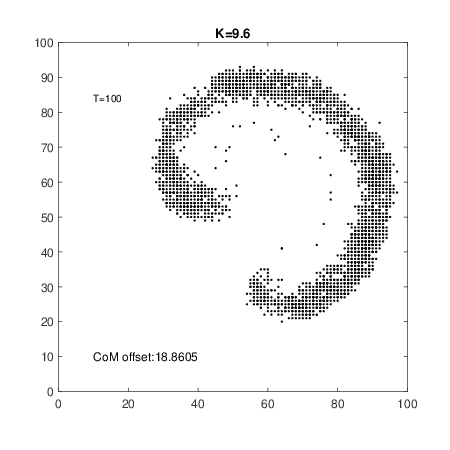
\includegraphics[width=0.45\textwidth]{fig/CoM_Example_K_9p5} }
     \subfloat[][]{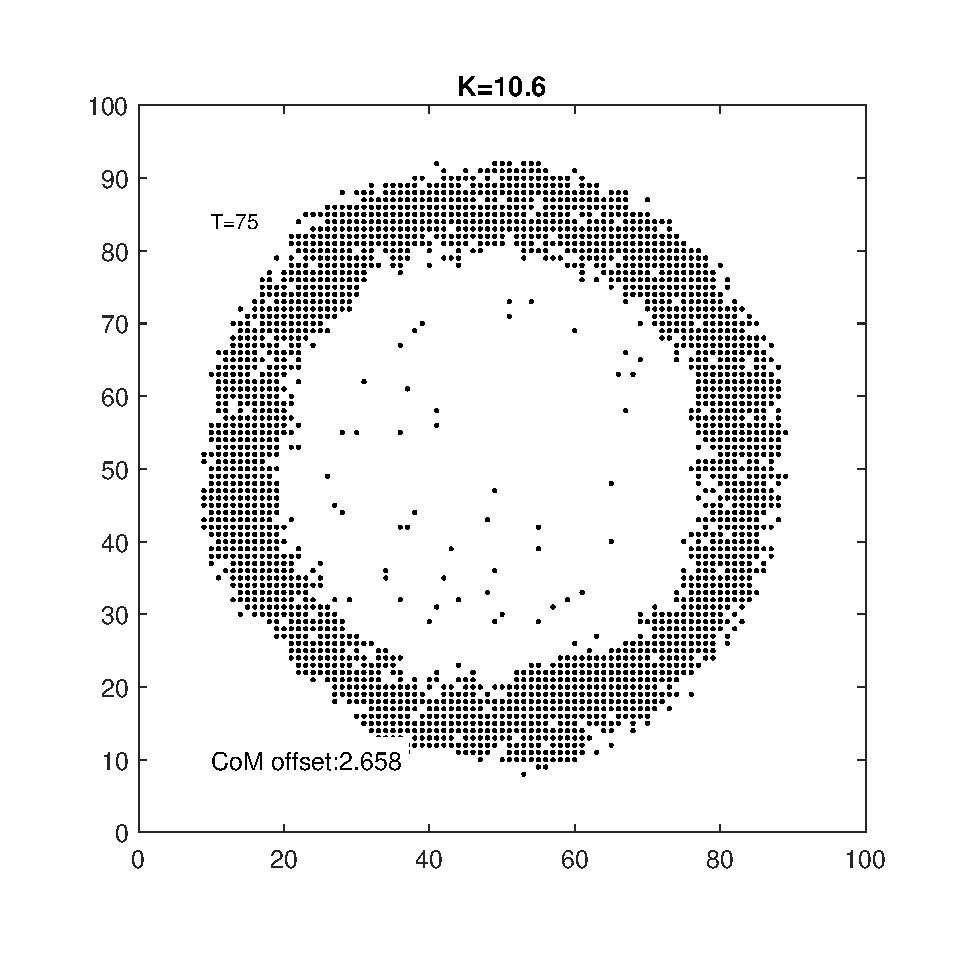
\includegraphics[width=0.45\textwidth]{fig/CoM_Example_K_10p5} }\\
     \subfloat[][]{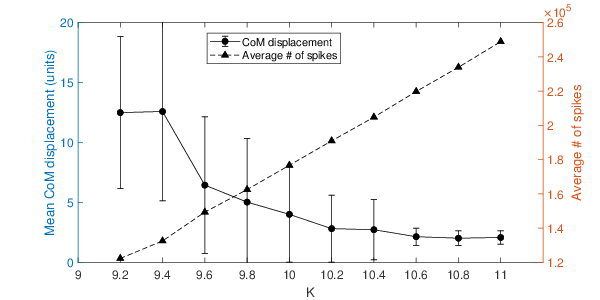
\includegraphics[width=0.75\textwidth]{fig/2DWaveTypeTransition} }
 \label{fig:2DWaveTransition}
\end{figure}
 \FloatBarrier

The waves in our simulations appear to create spatiotemporal patterns that repeat at some regular interval.
This is in contrast to \parencite{keane2015} who proposed traveling waves in 2-D sheets to explain why individual spike timing is highly irregular 
but membrane potential fluctuations can be correlated.
To compare our system to \parencite{keane2015} we calculate the coefficient of variation of the inter-spike intervals for the spiral wave experiment:

We examine the coefficient of variation and spike count cross-correlation for the simulation show in figure \ref{fig:2DSpiralWaves}.
As seen in figure \ref{fig:2DSpiralWave_SpikeTiming} the typical coefficient of variation is closer to 0 indicating highly regular firing.
This is in contrast with the simulated results in \parencite{keane2015} who observed highly irregular spiking in the individual neurons.
Our observation is qualitatively in agreement with voltage-sensitive dye experiments where any given pixel of the VSD image shows highly repetitive fluctuations (\parencite{Huang2010} figure 1, \parencite{huang2004} figure 2). 
The spike count correlation, when plotted as a function of the distance between neurons, shows that neurons that are closer together have more correlated activity.
This is in agreement with both simulated and observed traveling wave experiments.

\begin{figure}[!htb]
 \caption{Spike timing characterization of the spiral waves seen in figure \ref{fig:2DSpiralWaves}.
          a) The spike raster from a small number of neurons show regular spike events that correspond to passing waves.
          b) The histogram of all inter-spike intervals shows a peak $200~ms$ corresponding to the wave repetition rate. The peak near 0 is due to neurons firing several times when a wave passes. 
          c) The distribution of the coefficient of variation (eq. \ref{eq:cv}) confirms the regular spiking behavior as most of the CV values are near 0 (perfectly regular).
          d) The average correlation coefficient as a function of distance (\ref{eq:cross_correlation}) shows that the firing times of nearby neurons are highly correlated due to the wave structure.
          } 
     \subfloat[][]{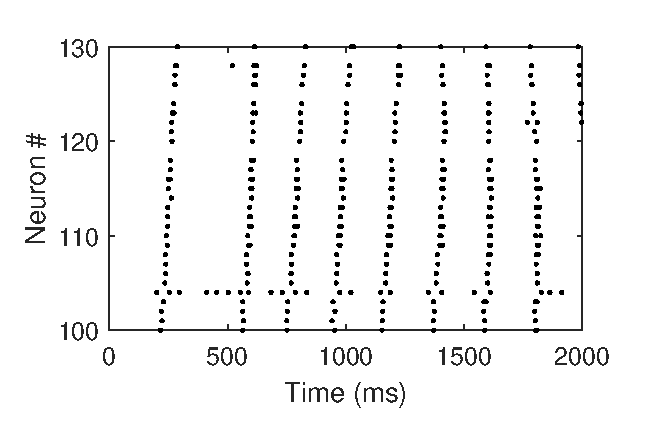
\includegraphics[width=0.48\textwidth]{fig/2DSpiralWaves_CorrelationRasterPlot} }
     \subfloat[][]{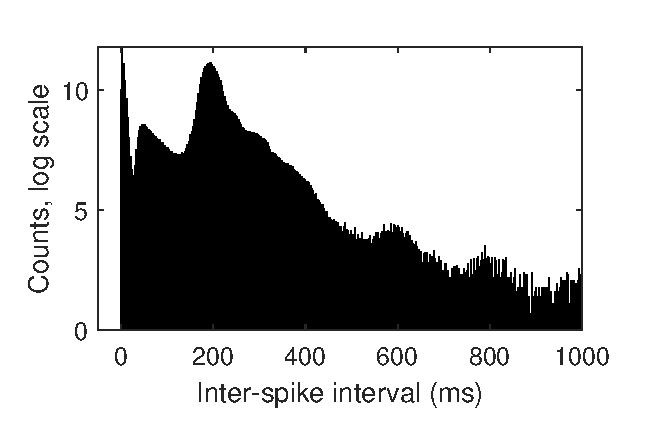
\includegraphics[width=0.48\textwidth]{fig/2DSpiralWaves_ISI_log} }\\
     \subfloat[][]{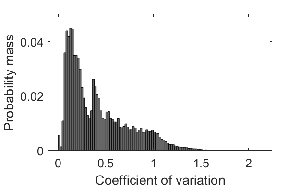
\includegraphics[width=0.48\textwidth]{fig/2DSpiralWaves_CVDist} }
     \subfloat[][]{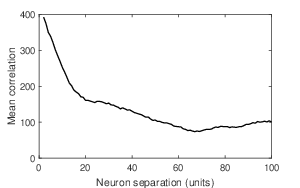
\includegraphics[width=0.48\textwidth]{fig/2DSpiralWaves_CorrelationCoefficient} }
 \label{fig:2DSpiralWave_SpikeTiming}
\end{figure}
 \FloatBarrier
 
This indicates that our 2D sheets exhibit spatiotemporal patterns that are both highly complex and yet repetitive over long time scales.
We consider a complex but repeating pattern as a dynamical attractor of the system.
To understand if the same system has multiple attractor states we compare multiple simulations of an identical system under different random stimulus.
\begin{figure}[!htb]
 \caption{ Another trial of the identical system from Figure \ref{fig:2DSpiralWaves}, but with a different random draw of the stimulus.
           The qualitative behavior is similar but the specific spatiotemporal pattern is clearly different.}
 \label{fig:2DSpiralWaves_SecondTrial}
 \centering
   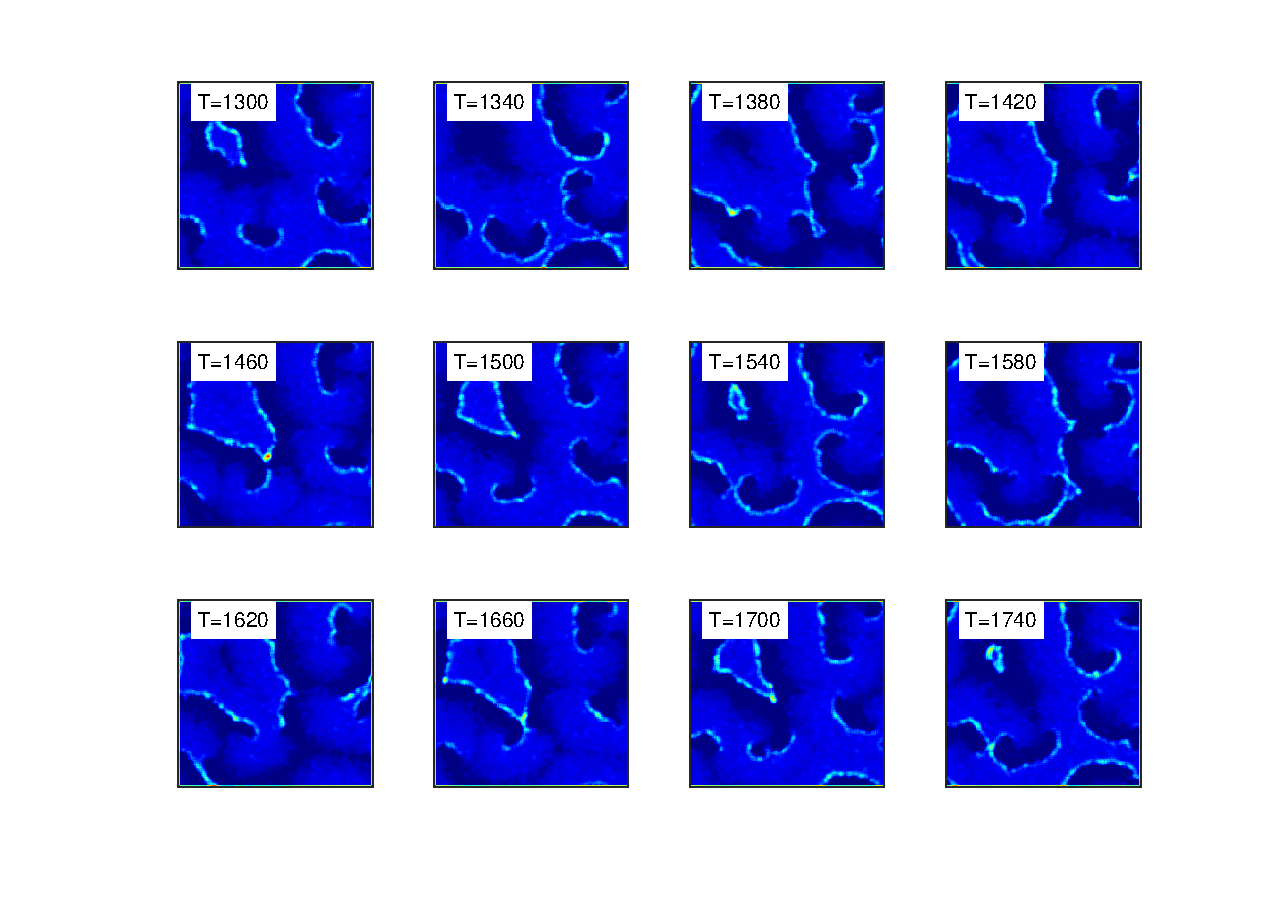
\includegraphics[width=\textwidth]{fig/SpiralWaves2D_K6_kappa0p1_M4_SecondTrial}
\end{figure}
\FloatBarrier

The traveling wave mechanism in the locally connected two dimensional sheet is the same as the locally connected one dimensional minicolumn.
We therefore expect similar traveling wave speeds, with the model parameters playing the same role as in the one dimensional minicolumn.
To measure speed in the sheet we extend the approach taken for the minicolumn by using an impulsive stimulus (equation ).
We use open boundary conditions when measuring wave speed in the two dimensional sheet.
We again find that we need to increase the connection strength $K$ when using an impulsive stimulus instead of a uniform background stimulus.
The neurons in the lower left corner near X=0, Y=0 are stimulated with a constant current for the first 10 milliseconds of the simulation.
This induces a circular spreading wave that spans the sheet as shown in figure \ref{fig:2DWaveSpeedRaster}.
The wave propagates isotropically with the same speed along both the X and Y axes.
The wave spans $100$ units in $192~ms$ for a speed of $0.52$ units/millisecond.
This is faster than the measured wave speed of $0.38$ units/millisecond in the minicolumn with the same model parameters.
Increasing the physical extents of our system increases the 
connectivity (figure \ref{fig:connection_delay_distrbution_2D}) leading to faster wave speeds.
\begin{figure}[!htb]
 \caption{ 2-D spike raster plots showing a single traveling wave.
           The sheet is 100x100x2 with model parameters at $\Sigma_v$ and $\kappa=1.0$.
           }
 \label{fig:2DWaveSpeedRaster}
 \centering
   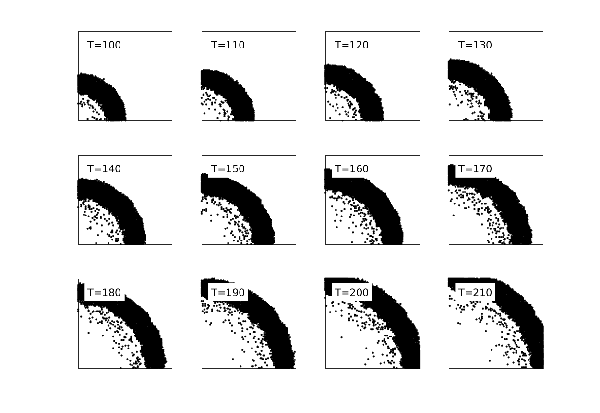
\includegraphics[width=\textwidth]{fig/2DWaveRasters_WaveSpeedExample}
\end{figure}
\FloatBarrier

The wave speed in our sheet depends on $\kappa$ (figure \ref{fig:2DWavePaceKappa}).
The lower y-intercept point in the sheet compared to the minicolumn indicates the lower pace (higher speed) due to the higher connectivity in the sheet.
\begin{figure}[!htb]
 \caption{ The pace of the wave depends linearly on $\kappa$.
           }
 \label{fig:2DWavePaceKappa}
 \centering
   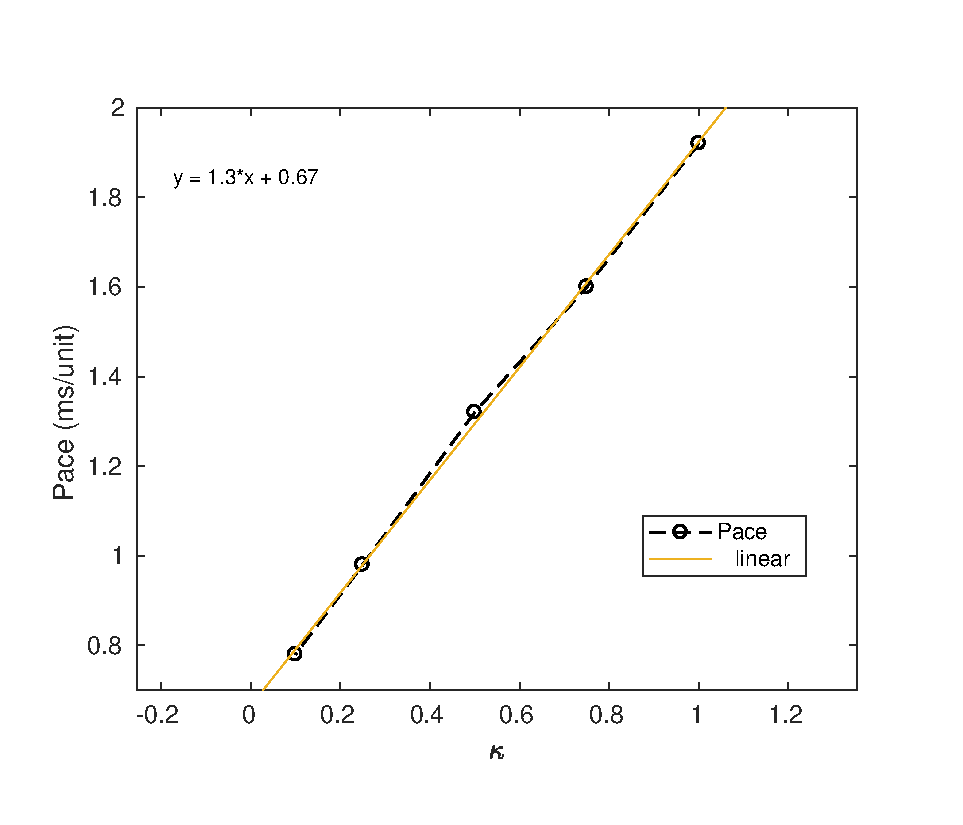
\includegraphics[width=0.5\textwidth]{fig/2DWavePace_Kappa}
\end{figure}
\FloatBarrier



\section{Discussion}
We have demonstrated traveling waves in quasi two-dimensional sheets with substantial spatial variation in the neurons and synapses.
Previous two-dimensional simulations using neural field models or leaky integrate-and-fire neurons addressed systems of identical neurons and isotropic connections.
In our model a purely two-dimensional system did not exhibit traveling waves, although it did exhibit spatial and temporal correlations in the neural activity.

We have shown that our model can exhibit the circular spreading waves, plane waves and spiral waves that are observed in the cortex.
The spiral waves are most prevalent at lower connection strengths.
We have shown that a single spreading wave can fracture into a spiral wave due to the variation in the underlying neural system.

Our quasi-2D sheets exhibit repeating spatio-temporal wave patterns.
These patterns are fairly stable over time and we consider them as attractor states of the system.
A given sheet can exhibit multiple attractor states, as applying different random background stimulus to the same sheet results in different wave patterns.

Previous work \parencite{keane2015} proposed traveling waves as an explanation for the seeming contradictions between the irregular spiking behavior of individual neurons 
and the correlation between the firing of nearby neurons.
We reproduce these results, showing substantial variance in the inter-spike intervals as well as higher correlation between the firing rates of nearby neurons.
We confirm that the neurons mostly fire when a traveling wave passes, but any individual neuron may not fire at all or fire multiple times when a particular wave passes.
We also find that for the special case of sparse connectivity our systems can exhibit extremely regular inter-spike intervals if each neuron fires only once when a wave passes.



\clearpage
\printbibliography

\end{document}
